%After conducting the measurements, profiles showing the drag and the drag coefficient as a function of Reynolds number could be created for each set of \gls{AD}s, as well as for the \gls{RWTM}s. 

During the measurement phase, it turned out that several measurement sets needed to be conducted for the rotating models, due to several deviations in the data. In this section, the measurement data and the process of treating it will be presented, together with the final average drag coefficient of the rotating models. After this, the drag and drag coefficient of all the different \gls{AD}s will be presented and compared to the average results for the rotating models.  

%In this section, the drag and drag coefficient profiles are presented and discussed, 

%as well as the calculated average Cd and the standard deviations. In the end, the measurement noise is discussed. 

\section{Rotating models}

The first measurement set conducted using three \gls{RWTM}s resulted in a drag coefficient that seemed relatively independent of Reynolds number for four of the measured Reynolds numbers, but with a noticeable deviation at $Re \approx 1.5*10^4$. To investigate whether this deviation was due to a measurement error, a second measurement set was conducted, this time using three new \gls{RWTM}s. This second measurement gave more of an expected result at $Re \approx 1.5*10^4$, however showed a deviation at $Re \approx 4.5*10^4$. Due to continuous deviations, however differing in size and appearing at different Reynolds numbers, six measurements were eventually conducted. They were all done with different sets of \gls{RWTM}s, except for measurement set three and four, which were done using the same set of models. The resulting drag coefficients can be seen as a function of Re in figure \ref{fig:RotationalCD}.

 

\begin{figure}
    \centering
    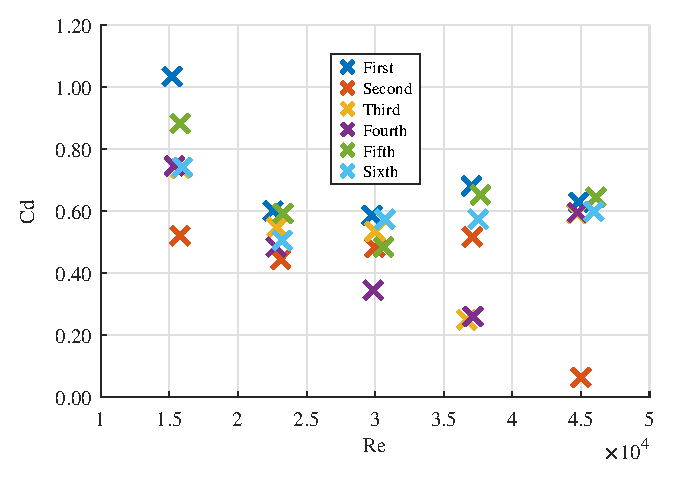
\includegraphics[width=0.8\linewidth]{0_Images/RotationalCDRe.eps}
    \caption[Drag coefficient for the rotating models.]{The drag coefficient for the rotating models, obtained through six rounds of measurements.}
    \label{fig:RotationalCD}
\end{figure}

As can be seen, there is some variation between the different measurements. The drag coefficients resulting from the third and the fourth measurement set, conducted using the same models, are quite similar at $Re \approx 1.5*10^4$, $Re \approx 2.3*10^4$ and $Re \approx 3.7*10^4$, and at $Re \approx 4.5*10^4$ they completely overlap. This seems to show that the measurement is to some degree repeatable, and that one of the reasons for the varying results is simply that there are small differences between the \gls{RWTM}s. These differences can for example be related to the friction between the rotating blades and the hub that they rotate around. In addition, the blades stay onto the hub due to a small piece of transparent plastic, that differs in size between the models. If it is too big, it might fasten the blades too tightly, causing added friction. If it is too small, the blades might be too loose, and they may start to oscillate. These types of differences were evident during the measurement phase, as several times the measurements had to be stopped midway due to one of the turbines suddenly not rotating anymore, and once because the rotating blades fell of the model.  

However, even between the third and fourth measurement set, there is a noticeable difference at $Re \approx 3*10^4$, showing that differences between the \gls{RWTM}s is not the only cause for the varying results. Other possible causes of this variation may be related to fluctuations in the applied wind velocity and to noise in the transducer and the electrical equipment used. Human error is also an important factor, as the models were placed in the wind tunnel by hand, and the turbine blades were not necessarily always exactly perpendicular to the incoming flow direction.   

To investigate the results further, the drag resulting from the different measurements were plotted as a function of Reynolds number, as seen in figure \ref{fig:RotationalDrag}.


\begin{figure}
    \centering
    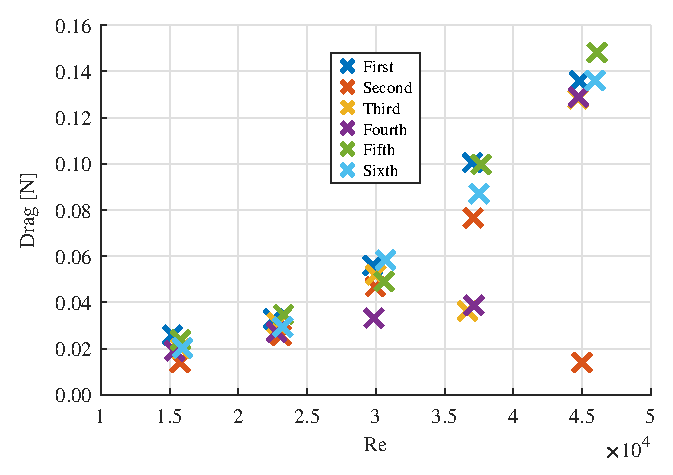
\includegraphics[width=0.8\linewidth]{0_Images/RotationalDragRe.eps}
    \caption[Drag for the rotating models.]{The measured drag for the rotating models, obtained through six rounds of measurements.}
    \label{fig:RotationalDrag}
\end{figure}

The drag at $Re \approx 4.5*10^4$ is significantly lower than the drag at $Re \approx 3.7*10^4$ for the second measurement set. The same is the case for the third measurement set, where the drag at $Re \approx 3.7*10^4$ is significantly lower than the drag at $Re \approx 3*10^4$. For the drag to decrease with increasing Re is not physical within this range of Reynolds numbers, and thus these two measurements are assumed to be outliers. 
%it is assumed that these two measurements are errors. 

The measurements at $Re \approx 3.7*10^4$ were studied further. By visual inspection there seems to be a cluster at around 0.09 \si{\N}, while the fourth measurement seems to be outside this cluster. This is confirmed by the fact that the distance between the fourth measurement and the mean of the cluster is over four times the standard deviation of the cluster. It is worth noting that this outlier is close to the already discarded drag measurement from the third measurement set. These two measurement sets used the same rotating models and both showed a considerable amount of noise on the signal for Reynolds numbers around $3.2*10^4-3.9*10^4$, which was not observed for the other measurement sets. Thus, these specific rotating models might be the reason for the repeated deviation at $Re \approx 3.7*10^4$.  

%The average drag of the measurements that seem to cluster is 0.091 \si{\newton}, with a standard deviation of 0.0114 \si{\newton}. Looking at the measurement value from the fourth measurement set, it has a drag of 0.0387 \si{\newton} at this Re, and thus it is over four standard deviations away from the mentioned average. Hence, this value is considered to be an outlier. 

%\todo{Should I comment on the fact that this outlier, discarded based on the fact that it was over four standard deviations away, almost coincides with another outlier, discarded in the previous paragraph based on the fact that the drag was decreasing with increasing velocity?}

%(It is worth noting that this outlier coincides with the already discarded drag measurement from the third measurement set. For these two measurement sets, using the same set of rotating models, there seemed to be considerably large amounts of noise on the signal for velocities between 11 \si{\m\per\s} and 13 \si{\m\per\s}, which might explain this repeated deviation.) 

%there seemed to be The wind tunnel seemed to produce considerably large amounts of noise on the signal for velocities between 11 and 13 \si{\m\per\s} for these two measurement sets that were conducted with the same set of rotating models, which might explain this repeated deviation.)
%The drag measured during the fourth measurement coincides with the disregarded drag from the third measurement, and is thus also regarded as an outlier. The wind tunnel did, for some unknown reason, seem to produce larger amounts of noise on the signal for velocities between 11 and 13 m/s for these specific measurement sets, which might explain this repeated deviation. 

A similar study was conducted for $Re \approx 3*10^4$. By visual inspection, five of the measurements seem to coincide at around 0.05 \si{\N}, while the fourth measurement seems to be outside this cluster. Once again, this is confirmed by the fact that the distance between the fourth measurement and the mean of the cluster is over four times the standard deviation of the cluster. 

%Five of the measurements seem to coincide, with an average drag of 0.0524 \si{\newton} and a standard deviation of 0.0047 \si{\newton}. The drag resulting from the fourth measurement set is 0.0332 \si{\newton}, and thus more than four standard deviations away from the average. Hence, this value is also considered to be an outlier.  

In total, four measured drags have been discarded, and the four associated drag coefficients were removed. In order to achieve a representative value for the drag coefficient of the \gls{RWTM}s, the average of the remaining drag coefficients was taken at each Reynolds number. This resulted in the drag coefficients seen in figure \ref{fig:RotationalAvg}. It is assumed that the drag measurements have a Gaussian distribution about some mean value, and that this calculated average based on six measurements is representative for the average one would have gotten if all the rotating models had been tested and all the tests had been conducted multiple times. It should be noted that this uncertainty related to the rotating models, causing the need for taking the average over several measurements, supports the claim that there is a need for alternative ways of modelling wind turbines. 


%The outlier seem to be spread out both in terms of velocity at which they occur and in terms of whether they exceed or fall below the other values. One can argue that if taking a large number of new measurements, they would have a Gaussian distribution about a mean, and that taking the average of the values that seemingly coincide would be representative for this total mean. %Should probably be extended 



\begin{figure}[h!]
    \centering
    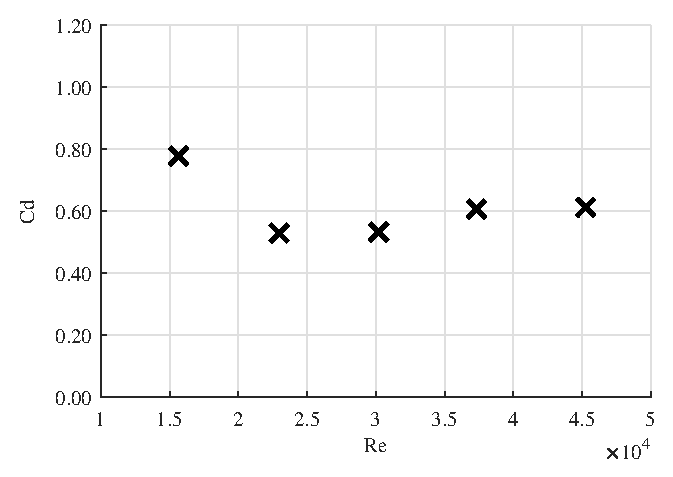
\includegraphics[width=0.8\linewidth]{0_Images/RotationalAverageRe.eps}
    \caption[Avergare drag coefficient for the rotating models.]{The average drag coefficient for the rotating models at each Reynolds number, based on the six conducted measurements, after removing the assumed errors and outliers.}
    \label{fig:RotationalAvg}
\end{figure}


%I BELIEVE THIS COMES LATER 
%Assuming that $C_d$ is Reynolds number independent for such a short span at Reynolds numbers, the average over these measurement points is taken, resulting in an average $C_d$ of 0.585. Based on all the applied values, the standard deviation at hand is... Thus, when creating the ADs, this is the desired drag coefficient. 

\FloatBarrier